% !Mode::"TeX:UTF-8"
\documentclass[a4paper, 11pt]{article}
\usepackage{amssymb}
\usepackage{geometry}
\usepackage{graphicx}
\usepackage{fancyhdr}
\usepackage{setspace}
\usepackage{pdfpages}
\usepackage{listings}
\usepackage{amsthm}
\usepackage{authblk}

\graphicspath{{./figure/}}

\geometry{left=2.5cm,right=2.5cm,top=2.5cm,bottom=2.5cm}

%\author{Chi Zhang\\\\Department of Computer Science\\\\University of Southern California}
\title{\textbf{Deep Learning for Short Term Portfolio Optimization}\\Project Proposal\thanks{Instructor: Joseph J. Lim}}
\author[]{Corey Chen}
\author[]{Chi Zhang}
\author[]{Limian Zhang\footnote{In alphabetical order}}
\affil[]{Department of Computer Science}


\begin{document}

  \maketitle                     %generate the title
  \begin{spacing}{1}
    \section{Problem Definition}
    In this project, we would like to optimize a short term portfolio based on the market. Concretely, we define $S$ as a set of stocks we want to invest. At timestamp 0, we have an initial investment volume of $M$ dollars and we don't hold any stocks. At timestamp $t$, we assume the stock we hold is $h_{p_1}, h_{p_2}, \cdots, h_{p_l}$. The action space at timestamp $t$ is $\{b_{i_1}, b_{i_2},\cdots, b_{i_n}, s_{j_1}, s_{j_2}, \cdots, s_{j_m}\}$, where each $b_{i_k}$ represents the amount we buy stock $i_k$, $k=1, 2, \cdots, n$ and each $s_{j_k}$ represents the amount we sell stock $j_k$, $k=1, 2, \cdots, m$. The action defined above is subject to $\sum_{k=1}^{n}b_{i_k}\leq M_t$, where $M_t$ is the investment volume at timestamp $t$. Also, $\{j_1, j_2, \cdots, j_m\}\subset\{p_1, p_2, \cdots, p_l\}$ and $s_{j_k}\leq h_{j_k}$, $k=1, 2, \cdots, m$. Assume the price of stock $i$ at timestamp $t$ is $P_{i, t}$, then $M_{t+1} = M_{t} - \sum_{k=1}^{n}b_{i_k} + \sum_{k=1}^{m}(P_{j_k, t} - \overline{B_{j_k}})$, where $B_{j_k}$ is the average price we buy for stock $j_k$ before timestamp $t$. 
    
    The problem is short term portfolio optimization. Thus, we constrain our investment to be in timestamp $0, 1, \cdots, T$ and the goal is to maximize the investment volume at timestamp $T$.
    
    Since we are modeling real world market trades, we make several assumptions to simplify the problems:
    \begin{itemize}
      \item We can get any information about the stocks before timestamp $t$ for stock $i$. e.g. The previous stock price, the news and tweets online.
      \item Our investment will not change how the market behaves. That is, we can do it in a fully supervised manner instead of using adversarial and reinforcement learning.
      \item At timestamp $t+1$, the stock price of all previous timestamps become ground truth. This means we can adjust our model along with the investment.
    \end{itemize}
    
    \section{Methods and Datasets}
    
    \begin{figure}
      \centering
      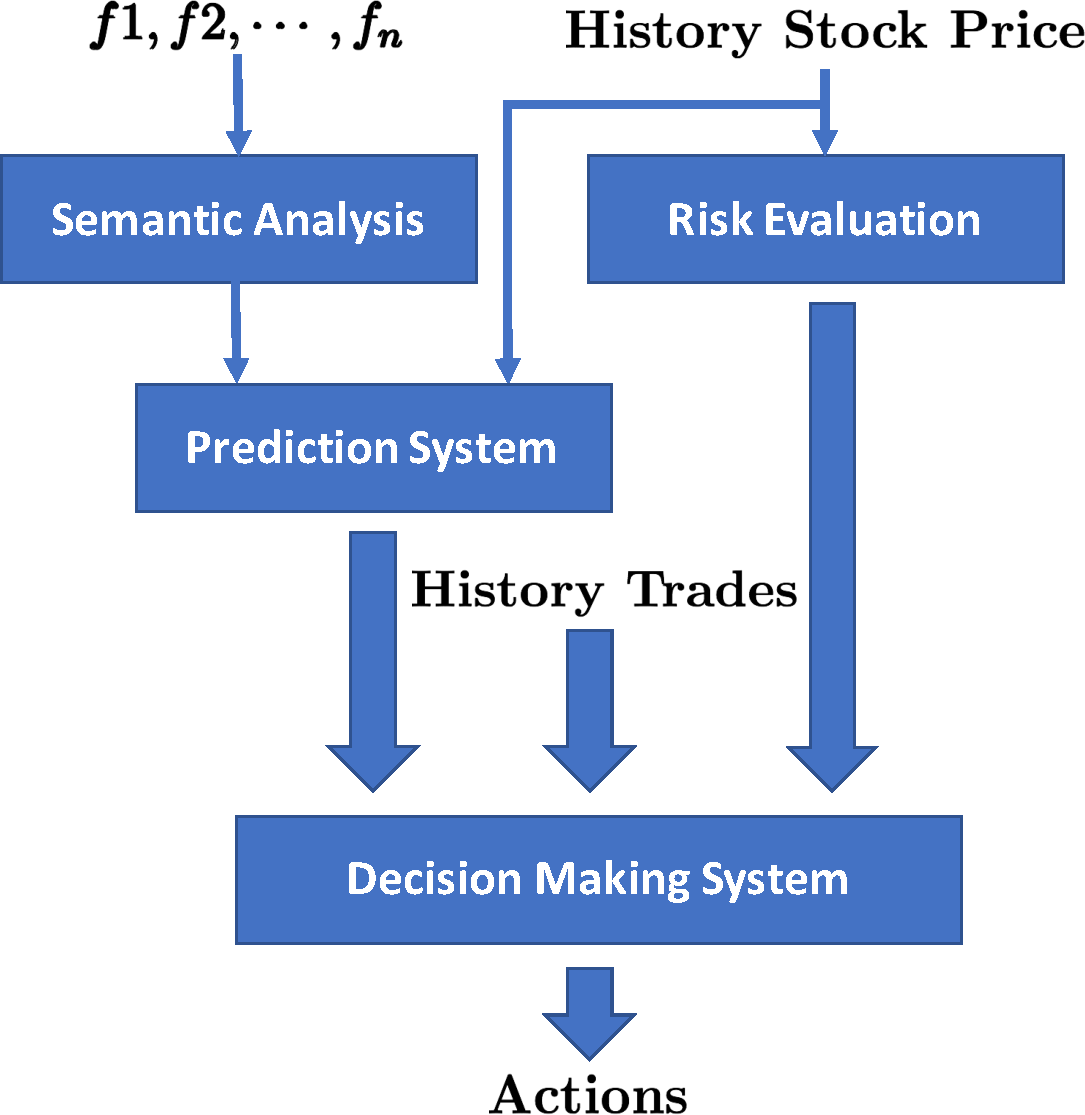
\includegraphics[width=0.5\textwidth]{diagram}
      \caption{Digram of proposed approach}
      \label{diagram_approach}
    \end{figure}
    
    The diagram of our approach is shown in Figure~\ref{diagram_approach}. It has been studied in \cite{social_relation_sentiment_analysis} that social sentiments reflect how stock market behaves. Besides, we assume the stock price follows certain statistics before big news happens. We devide our system into three subsystems:
    \begin{enumerate}
      \item Semantic Analysis: We parse the tweets of $n$ stocks $f_1, f_2, \cdots, f_n$ and produce a score for each stock $s_1, s_2, \cdots, s_n$, representing the expected ratio of price increase or decrease.
      \item Prediction: We take the scores provided by Semantic Analysis and combine with the history price to produce the predicted value of a stock.
      \item Risk Evaluation: To measure the risk, we consider the variance of our predicted price. We evaluate the variance by the accuracy of the prediction history.
      \item Decision Making: With the predicted price, risk evaluation and our history trades, we produce the final actions.
    \end{enumerate}
    Note that details of each sub-system is not decided yet. They can be a single neural network or more complicated structure. Or the whole system can be trained end-to-end. Our baseline is reinforcement learning based approach done in \cite{cs229_stanford_trading, cs229_stanford_portfolio}.
%    
%    \section{Related Work}
%    \cite{cs229_stanford_portfolio}
%    
%    \section{Milestones}
%    
%    \section{Potential Problems} 
  
  \end{spacing}  
  \bibliographystyle{abbrv}
  \bibliography{./bib/stock_prediction.bib}

\end{document}
